\section{Results}
In this section, we study PSF size and ellipticity residuals as a function of magnitude, sky position (DCR), and colour. 
We use the week 49 DRP data, which contains 4898 visits and $\sim$ 153 million star measurements. 
We perform the measurements using all stars, and we use stars binned by $r-z$ colour in 3 equally distributed bins to quantify the colour-dependent effects. 
We show how the PSF model improves when enabling chromatic fitting of the PSF in \texttt{PiFF}.


\subsection{Residuals by magnitude}

\begin{figure}[h!]
  \centering

  \begin{subfigure}{\textwidth}
    \centering
    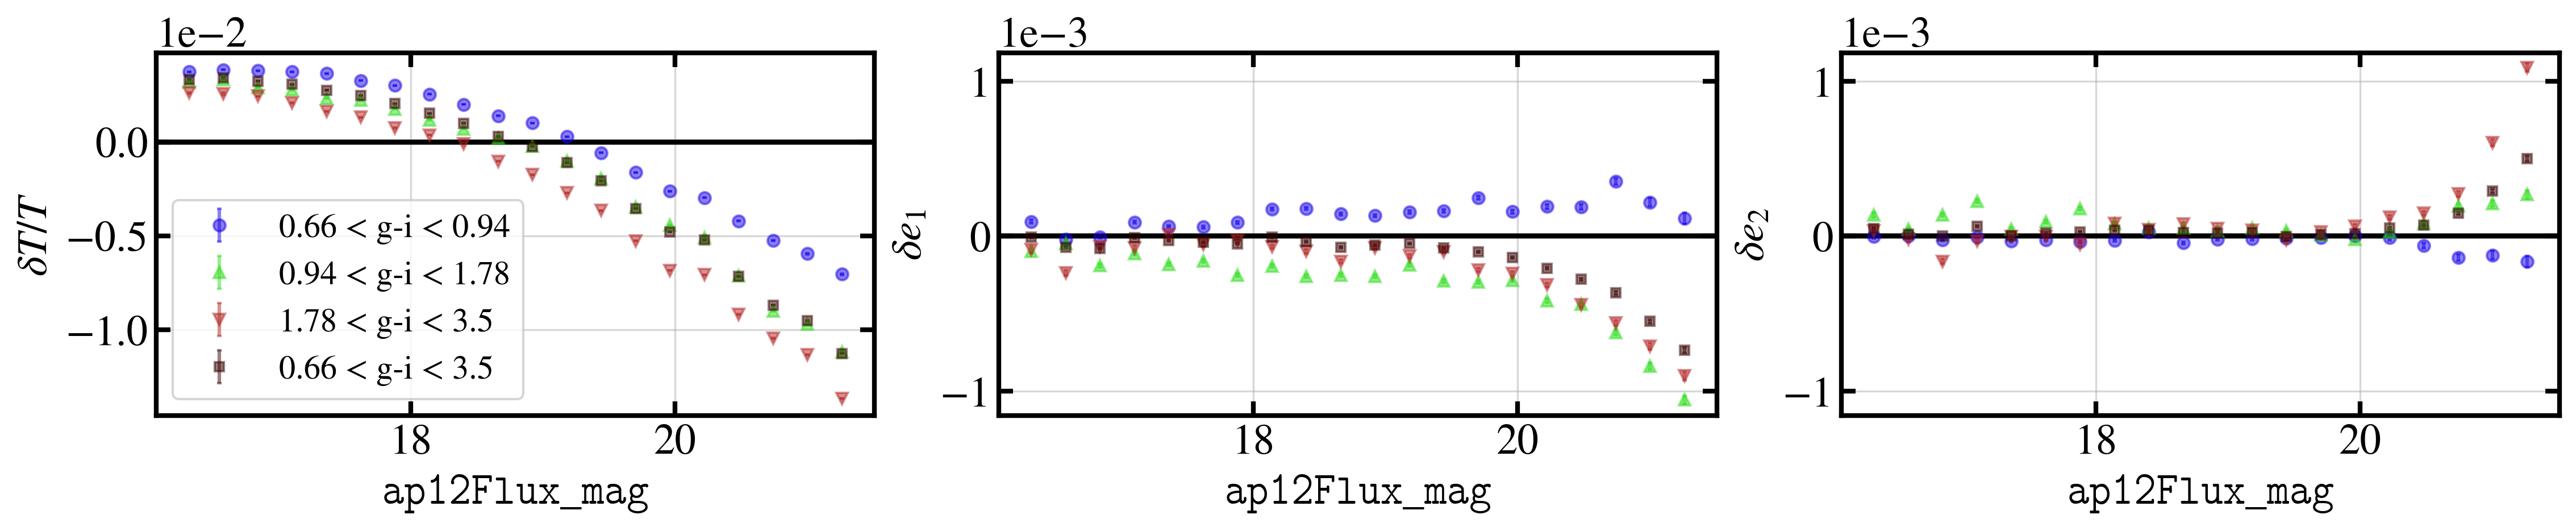
\includegraphics[width=1\textwidth]{figures/color_separated_residuals_vs_calibfluxmag_no_correction.png}
    \caption{without chromatic PSF fitting.}
  \end{subfigure}
  \medskip
  \begin{subfigure}{\textwidth}
    \centering
    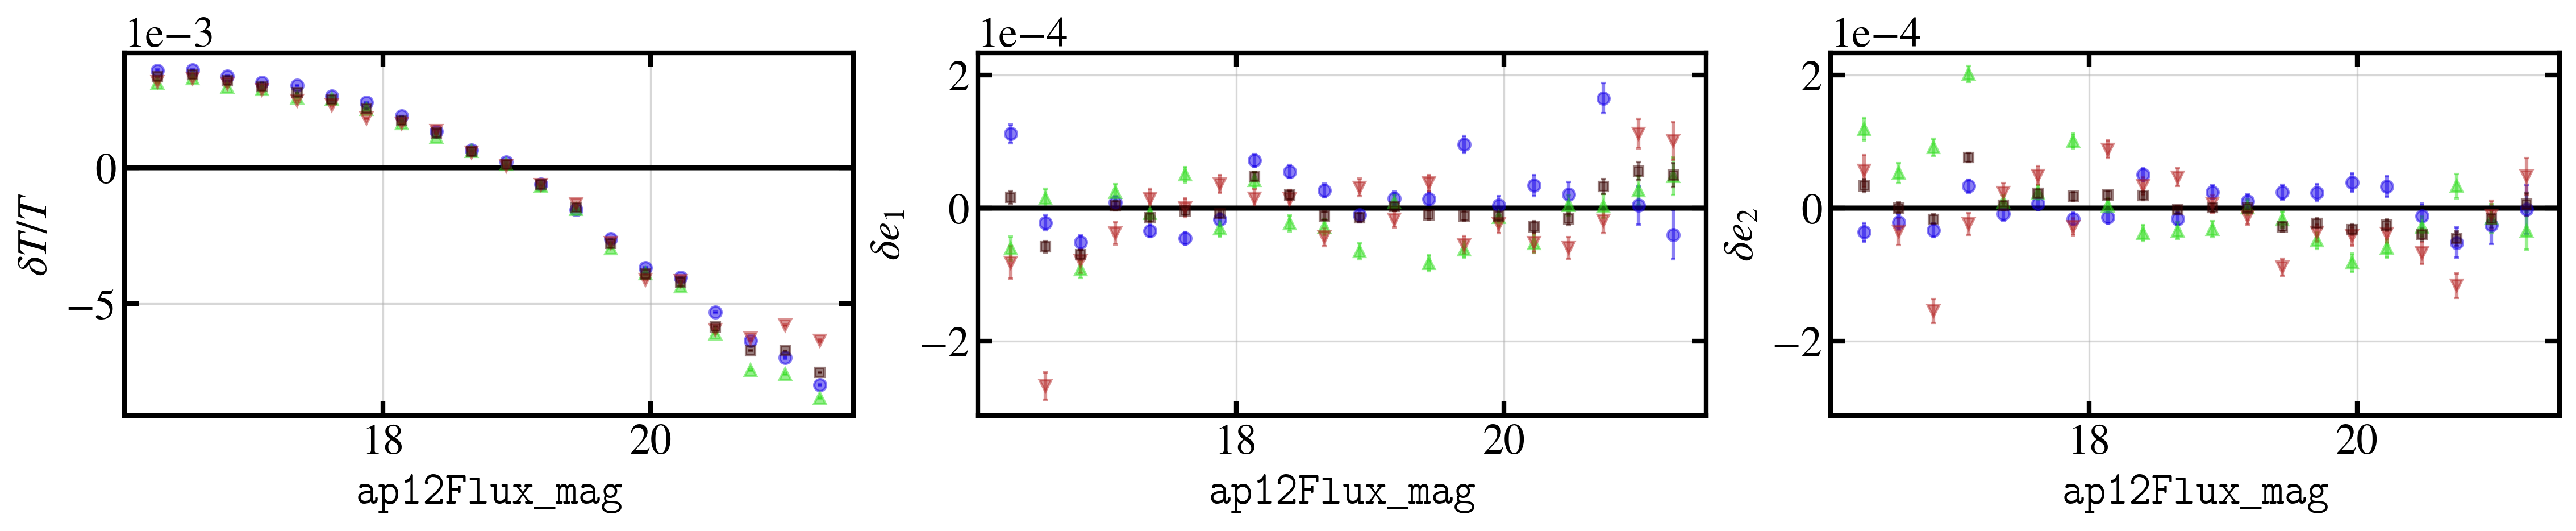
\includegraphics[width=1\textwidth]{figures/color_separated_residuals_vs_calibfluxmag_with_correction.png}
    
    \caption{with chromatic PSF fitting.}
    \label{subfig:residuals_vs_mag_b}
  \end{subfigure}

  \caption{PSF $\delta T/T$, $\delta e_1$ and $\delta e_2$ as a function of \texttt{ap12Flux\_mag} before (a) and after (b) turning on chromatic PSF fitting. 
  Note that the y-axis range in (a) and (b) are different. Stars are divided into equal-sized colour bins of $r-z \in [0.25, 0.38, 0.82, 3.5]$. 
  Enabling chromatic PSF reduces the spread or residuals between colour bins. }
  \label{fig:residuals_vs_mag}
\end{figure}

Figure~\ref{fig:residuals_vs_mag} shows the PSF $\delta T/T$, $\delta e_1$ and $\delta e_2$ residuals as a function of star magnitude. 
The stars have been divided into colour bins of $r-z \in [0.25, 0.38, 0.82, 3.5]$. 
Without chromatic fitting, the spread in $\delta e_{1}$ at the faint end is $\sim 3\times$ larger than that of $\delta e_{2}$. 
Enabling chromatic fitting of the PSF tightens and thereby reduces the spread in the residuals toward the faint end in all colour bins, but is most prominently seen in $\delta e_{1}$.
As expected, the magnitude of the errors are not reduced by chromatic fitting, but the spread between the individual colour bins is reduced, which can be most clearly seen in $\delta T/T$. 

Figure~\ref{fig:residuals_vs_mag_g} shows the residuals of PSF $\delta T/T$, $\delta e_1$ and $\delta e_2$ as a function of star magnitude for visits in the $g$ band only, where we expect to see the most significant chromatic PSF effect. 
%The discrepancy between the residuals in each colour bin is the largest for visits in the $g$ band.
The stars are divided into colour bins of $r-z \in [0.24, 0.35, 0.57, 3.5]$. 
Enabling chromatic fitting reduces $\delta T/T$ residuals by $\sim$ 50\%.
For $\delta e_{1}$ and $\delta e_{2}$, chromatic fitting tightens the residuals at the faint end (mag > 18) by $\sim$ 75\%.
It is comparatively ineffective in tightening the reddest colour bin at the bright end.


\begin{figure}[h!]
  \centering

  \begin{subfigure}{\textwidth}
    \centering
    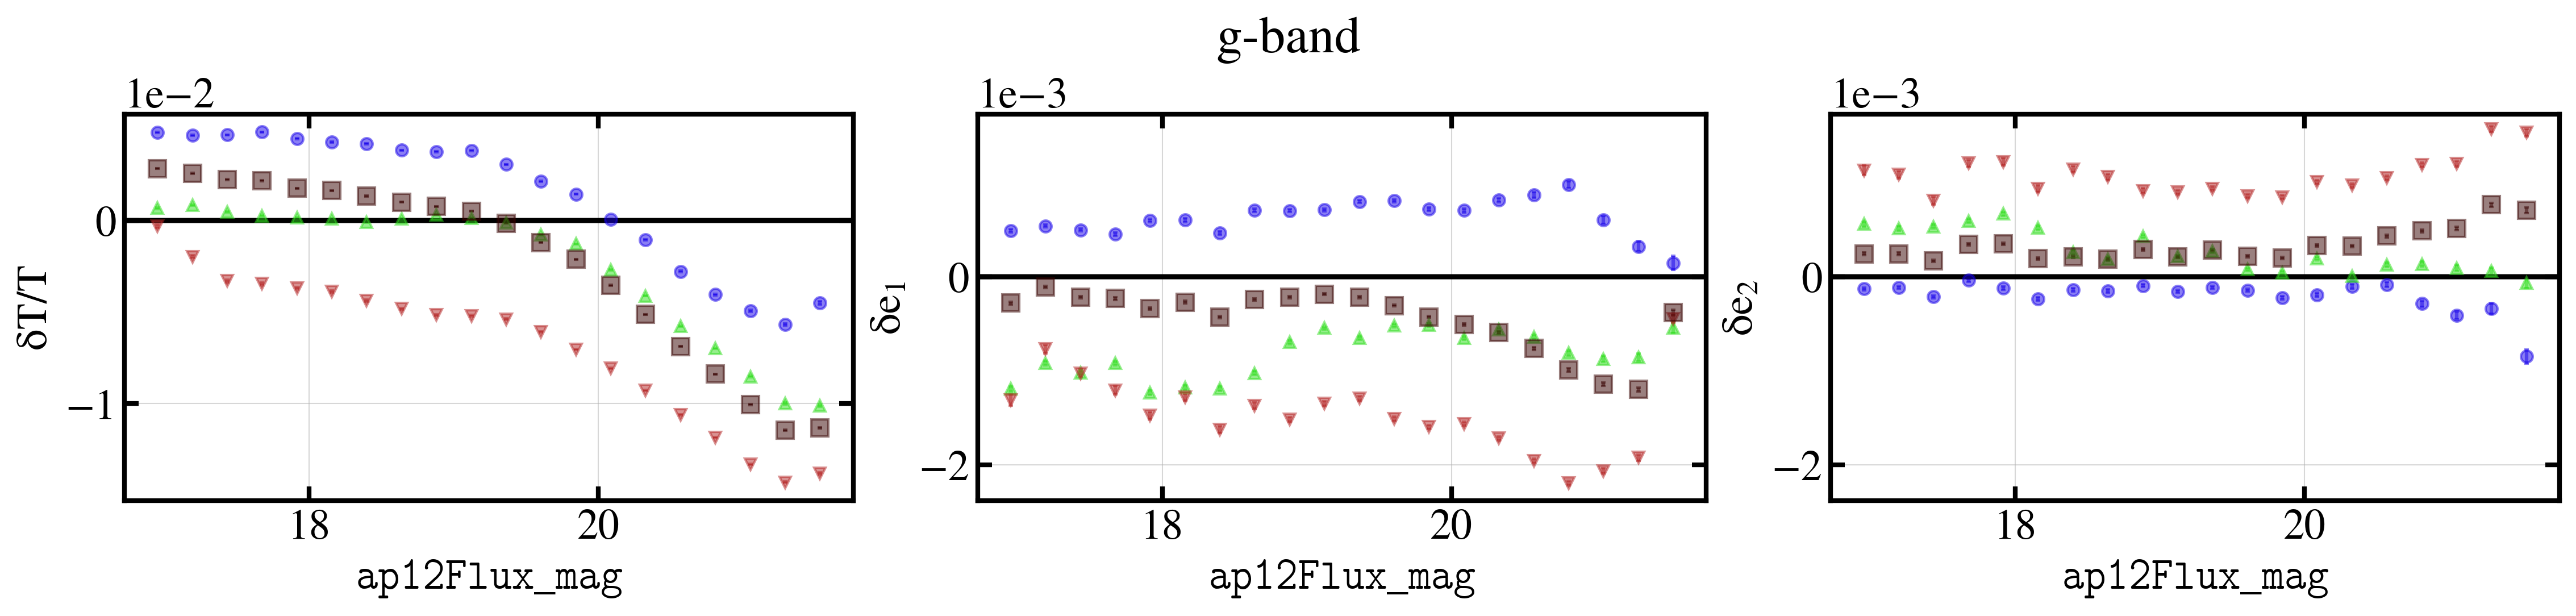
\includegraphics[width=1\textwidth]{figures/color_separated_residuals_vs_calibfluxmag_no_correction_g_band.png}
    \caption{without chromatic PSF fitting.}
  \end{subfigure}
  \medskip
  \begin{subfigure}{\textwidth}
    \centering
    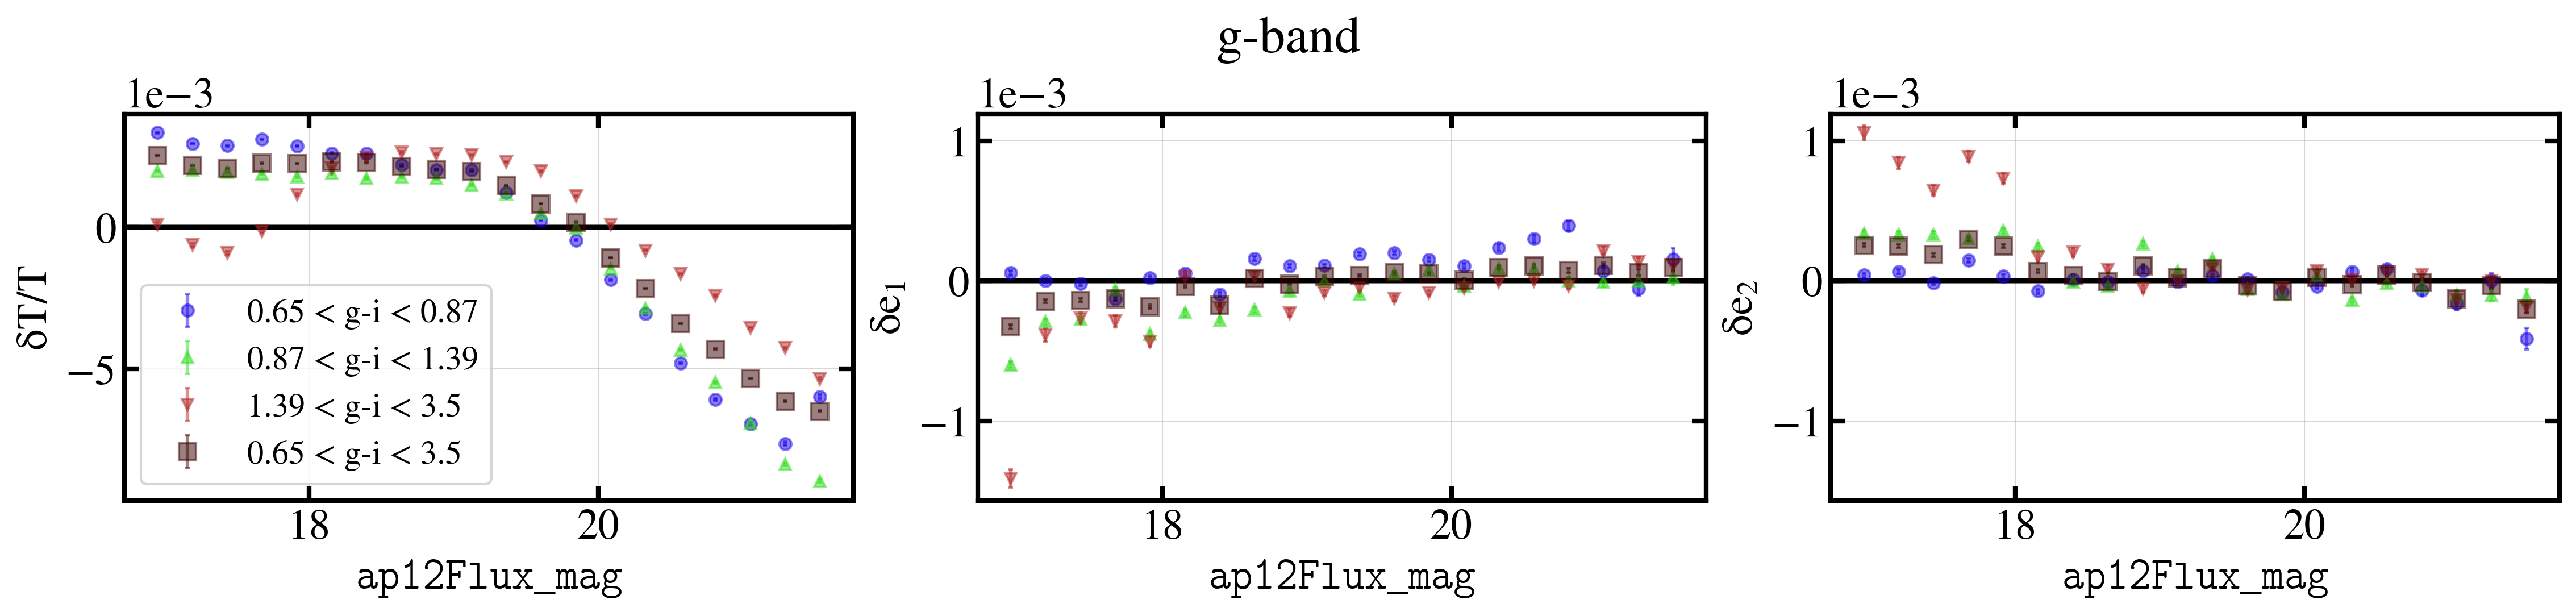
\includegraphics[width=1\textwidth]{figures/color_separated_residuals_vs_calibfluxmag_with_correction_g_band.png}
    \caption{with chromatic PSF fitting.}
    
  \end{subfigure}

  \caption{PSF $\delta T/T$, $\delta e_1$ and $\delta e_2$ for $g$ band visits only as a function of \texttt{ap12Flux\_mag} before (a) and after (b) turning on chromatic PSF fitting. 
  Note that the y-axis range in (a) and (b) are different. Stars are divided into equal-sized colour bins of $r-z \in [0.24, 0.35, 0.57, 3.5]$. 
  Enabling chromatic PSF shows the most improvement in the residuals in the blue, faint objects.}
  \label{fig:residuals_vs_mag_g}
\end{figure}

\subsection{Residuals by colour}

Figure~\ref{fig:residuals_vs_colour} plots the PSF $\delta T/T$, $\delta e_1$ and $\delta e_2$ residuals as a function of $g-i$ colour.
The right-most panel of subfig.~\ref{subfig:color_vs_residuals_b} shows the number density of stars as a function of $g-i$ colour, which is common to both subfigures.
The residuals of $\delta T/T$ and $\delta e_{1}$ show the strongest colour dependence in the $u$ and $g$ bands respectively.
Chromatic fitting corrects the colour dependence in the $g$ band, but is ineffective in correcting the $u$ band colour dependence.
However, this could be due to the lack of enough objects in the $u$ band in red $g-i$ bins, as can be seen in the histogram.
The discrepancy between the magnitude of $\delta e_1$ and $\delta e_2$ residuals is also unclear.
\begin{figure}[h!]
  \centering

  \begin{subfigure}{\textwidth}
    \centering
    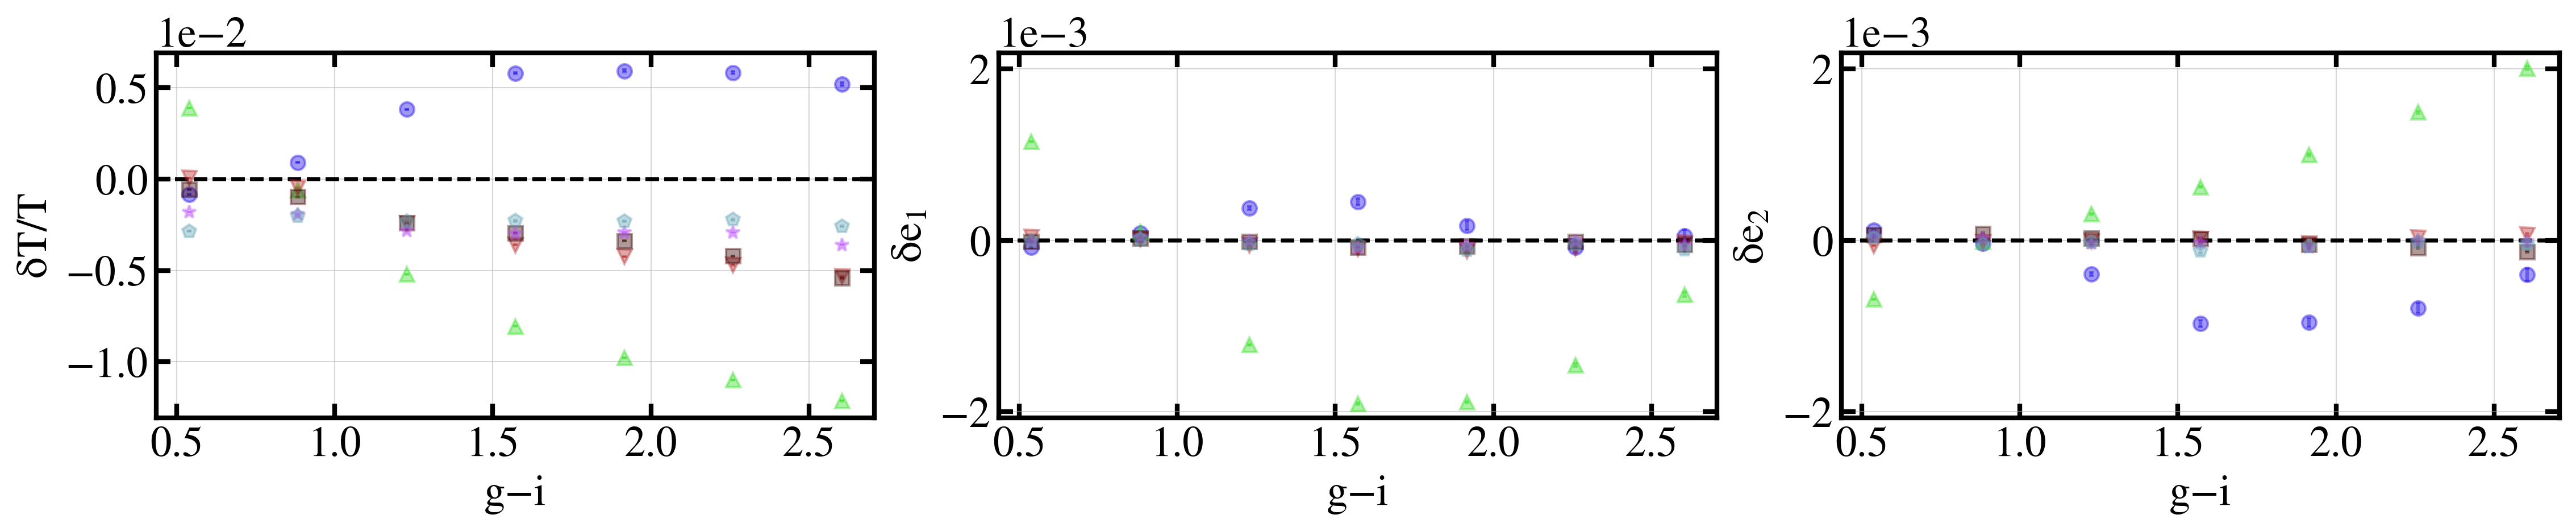
\includegraphics[width=1\textwidth]{figures/residuals_vs_gmi_color_no_correction.png}
    \caption{without chromatic PSF fitting.}
  \end{subfigure}
  \medskip
  \begin{subfigure}{\textwidth}
    \centering
    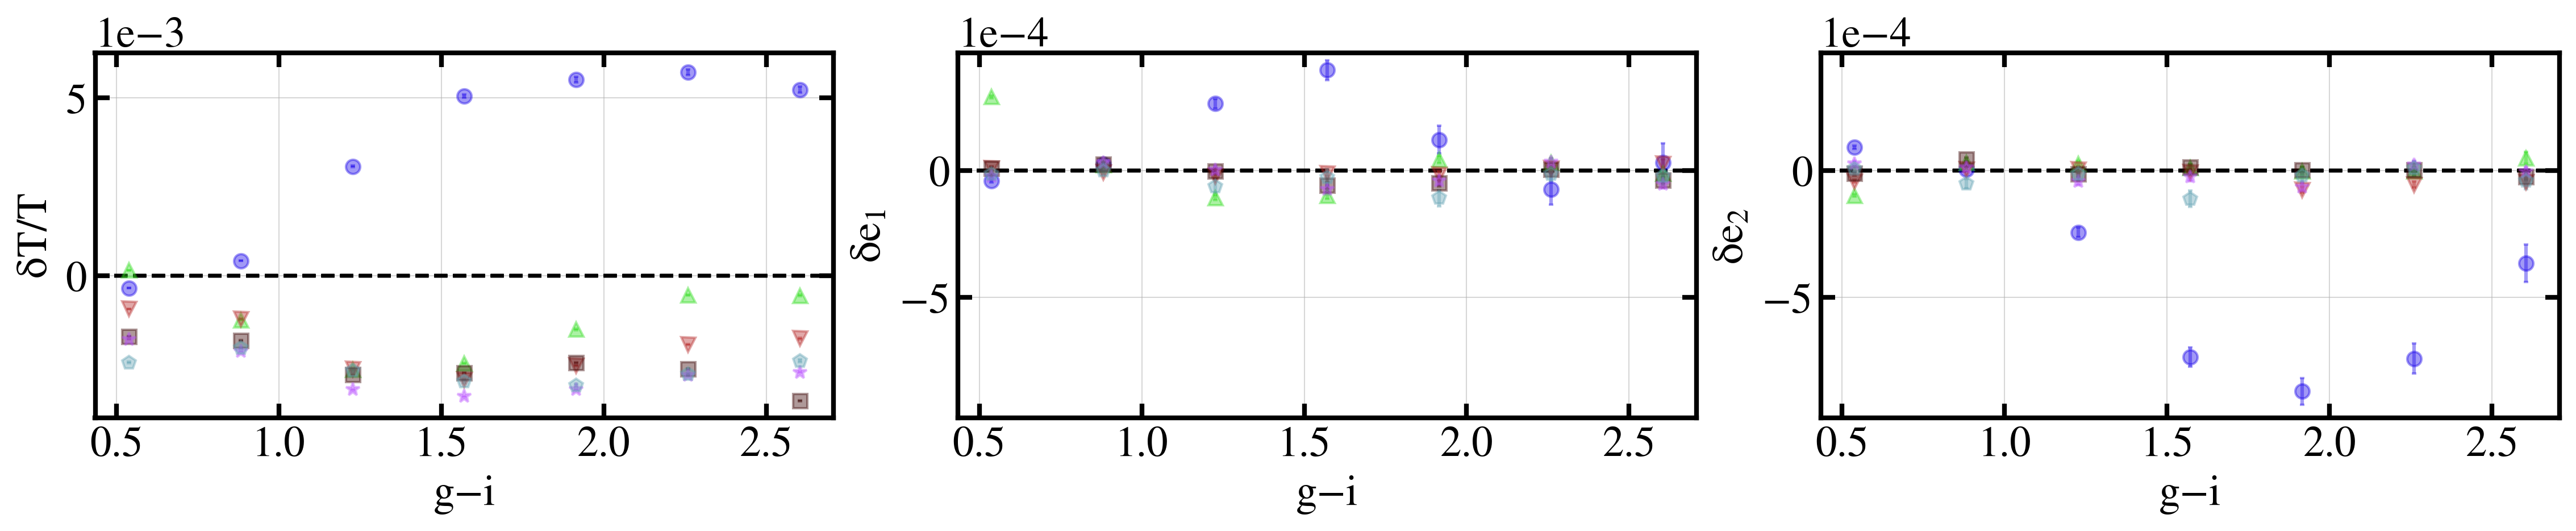
\includegraphics[width=1\textwidth]{figures/residuals_vs_gmi_color_with_correction.png}
    \caption{with chromatic PSF fitting.}
    \label{subfig:color_vs_residuals_b}
  \end{subfigure}

  \begin{subfigure}{\textwidth}
    \centering
    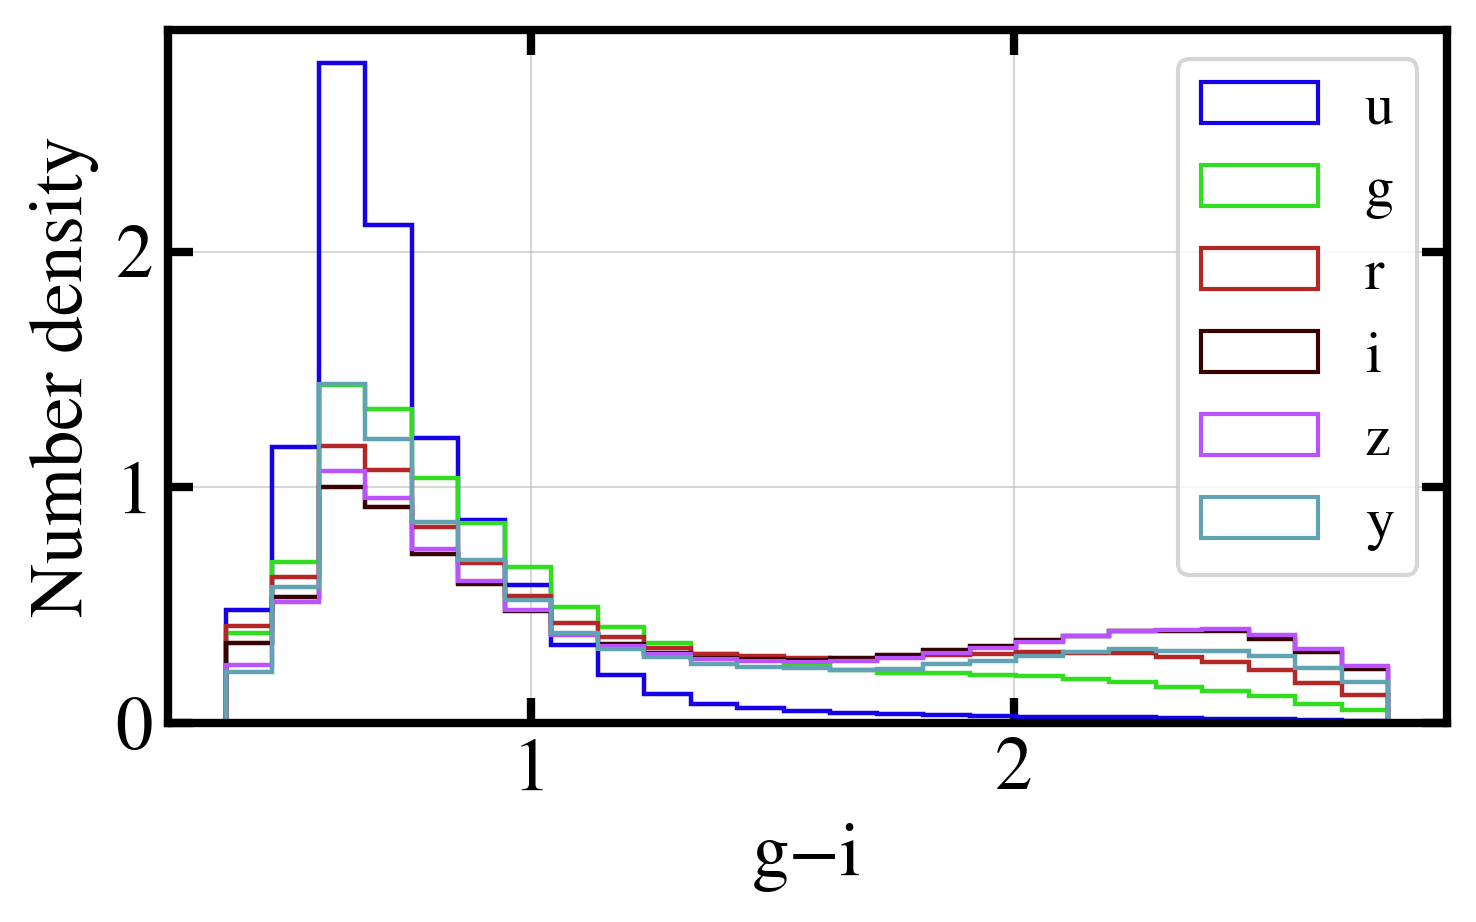
\includegraphics[width=0.3\textwidth]{figures/color_hist.png}
    \caption{Number density as a function of $g-i$ colour.}
    \label{subfig:color_vs_residuals_c}
  \end{subfigure}

  \caption{PSF $\delta T/T$, $\delta e_1$ and $\delta e_2$ as a function of $g-i$ colour. 
  The $u$ and $g$ band residuals show the highest dependence on $g-i$ colour. 
  Note that the y-axis range in (a) and (b) are different.
  Enabling chromatic fitting corrects the $g$ band colour dependence, but is unable to correct the $u$ band dependence, possibly due to the small number of observations with red $g-i$ colour. }
  \label{fig:residuals_vs_colour}
\end{figure}

\subsection{Residuals by Position (DCR)}

Figure~\ref{fig:g_dcr} shows the PSF $\delta e_{1}$ and $\delta e_{2}$ as a function of $\mathrm{DCR_1}$ and $\mathrm{DCR_2}$ respectively for observations in the $g$ band, which is affected the most by DCR.
The stars are separated in colour bins of $r-z \in [0.25, 0.38, 0.82, 3.5]$.
Chromatic fitting of the PSF corrects DCR dependent residuals by up to $\sim$ 90\% in $\delta e_{1}$ and up to $\sim$ 95\% in $\delta e_{2}$, therefore reducing DCR dependent errors by almost an order of magnitude.

\begin{figure}[h!]
  \centering

  \begin{subfigure}[t]{0.45\textwidth}
    \centering
    \includegraphics[width=\linewidth]{figures/shape_residuals_vs_dcr_no_correction_g.png}
    \caption{without chromatic PSF fitting.}
    \label{subfig:g_dcr_a}
  \end{subfigure}
  \hfill
  \begin{subfigure}[t]{0.45\textwidth}
    \centering
    \includegraphics[width=\linewidth]{figures/shape_residuals_vs_dcr_with_correction_g.png}
    \caption{with chromatic PSF fitting.}
    \label{subfig:g_dcr_b}
  \end{subfigure}

  \caption{PSF $\delta e_1$ and $\delta e_2$ as a function of $\mathrm{DCR_1}$ and $\mathrm{DCR_2}$ respectively  before (a) and after (b) turning on chromatic PSF fitting. 
  Note that the y-axis range in (a) and (b) are different.
  Chromatic fitting of the PSF reduces residuals by up to $\sim$ 95\% in the $g$-band.}
  \label{fig:g_dcr}
\end{figure}

\begin{figure}[h!]
  \centering

  \begin{subfigure}[t]{0.45\textwidth}
    \centering
    \includegraphics[width=\linewidth]{figures/shape_residuals_vs_dcr_no_correction_r.png}
    \caption{without chromatic PSF fitting.}
    \label{subfig:r_dcr_a}
  \end{subfigure}
  \hfill
  \begin{subfigure}[t]{0.45\textwidth}
    \centering
    \includegraphics[width=\linewidth]{figures/shape_residuals_vs_dcr_with_correction_r.png}
    \caption{with chromatic PSF fitting.}
    \label{subfig:r_dcr_b}
  \end{subfigure}

  \caption{PSF $\delta e_1$ and $\delta e_2$ as a function of $\mathrm{DCR_1}$ and $\mathrm{DCR_2}$ respectively  before (a) and after (b) turning on chromatic PSF fitting. 
  Note that the y-axis range in (a) and (b) are different.
  Chromatic fitting of the PSF reduces residuals by up to $\sim$50\% in the $r$-band.}
  \label{fig:r_dcr}
\end{figure}

Figure~\ref{fig:r_dcr} shows the PSF $\delta e_{1}$ and $\delta e_{2}$ as a function of $\mathrm{DCR_1}$ and $\mathrm{DCR_2}$ respectively for observations in the $r$ band.
The stars are separated in colour bins of $r-z \in [0.25, 0.38, 0.82, 3.5]$.
Chromatic fitting of the PSF corrects DCR dependent residuals by up to $\sim$ 50\% in $\delta e_{1}$ and $\delta e_{2}$.

